%! Author = natalia
%! Date = 15.01.2020

% Preamble
\documentclass{beamer}

\mode<presentation>
{
\usetheme{Warsaw}
% or Goettingen or Malmoe
\setbeamercovered{transparent}
% or whatever (possibly just delete it)
%\usecolortheme{seahorse}
}



% Packages
\usepackage[english]{babel}
\usepackage[utf8]{inputenc}
%\usepackage{times}
%\usepackage[T1]{fontenc}
\usepackage{amsthm}
\usepackage{graphicx}



\title{An Introduction to Concurrency in Python}
\author{Natalia Maniakowska}
\institute{skygate}
\date{16-01-2020}

%\pgfdeclareimage[height=0.5cm]{company-logo}{skygate_logo.jpg}
%\logo{\pgfuseimage{company-logo}}

%\AtBeginSubsection[]
%{
%\begin{frame}
%    <beamer>{Outline}
%    \tableofcontents[currentsection,currentsubsection]
%\end{frame}
%}

\beamerdefaultoverlayspecification{<+->}

% Document
\begin{document}

    \frame{\titlepage}

    \begin{frame}{Outline}
        \tableofcontents
        % You might wish to add the option [pausesections]
    \end{frame}


    %%%%%%%%%%%%%%%%%%%%%%%%%%%%%%%%%%%%%%%%%%%%%%%%
    \section{Introduction}

    \subsection{Definitions}


    \begin{frame}
        \frametitle{What is concurrency, actually?}

        \begin{itemize}
            \item Medieval Latin \emph{concurrentia} "a running together"

            (cf. English \emph{current}, \emph{concur})
            \item so: simultaneous occurrence\dots
            \item \dots but is it \textbf{really} simultaneous? What does is mean, anyway?

        \end{itemize}

    \end{frame}

    \begin{frame}
        \frametitle{Concurrency vs. Parallelism}
        \framesubtitle{https://wiki.haskell.org/Parallelism\_vs.\_Concurrency}

        \textbf{Disclaimer:} Not all programmers agree on the meaning!


        \begin{definition} A \textbf{parallel program} is one that uses a multiplicity of
        computational hardware (e.g. multiple processor cores) in order to perform
        computation more quickly. Different parts of the computation are delegated
        to different processors that execute at the same time (in parallel).

        \end{definition}

        \begin{definition} \textbf{Concurrency} is a program-structuring technique
        in which there are multiple threads of control. The user sees their effects interleaved.
        Whether they actually execute at the same time or not is an implementation detail.

        \end{definition}

    \end{frame}


    \subsection{Different Types of Concurrency -- More Details}

    \begin{frame}
        \frametitle{CPU-bound tasks: multiprocessing/parallel processing}

        \begin{itemize}
            \item Simultaneous. Like, really simultaneous!
            \item Multiple processes, multiple CPU cores
            \item Good for: matrix multiplications, searching, image processing, etc.
            \item Problems: computation parallelization, sending data between processes
        \end{itemize}

    \end{frame}

    \begin{frame}
        \frametitle{CPU-bound tasks -- continued}

        \begin{figure}
            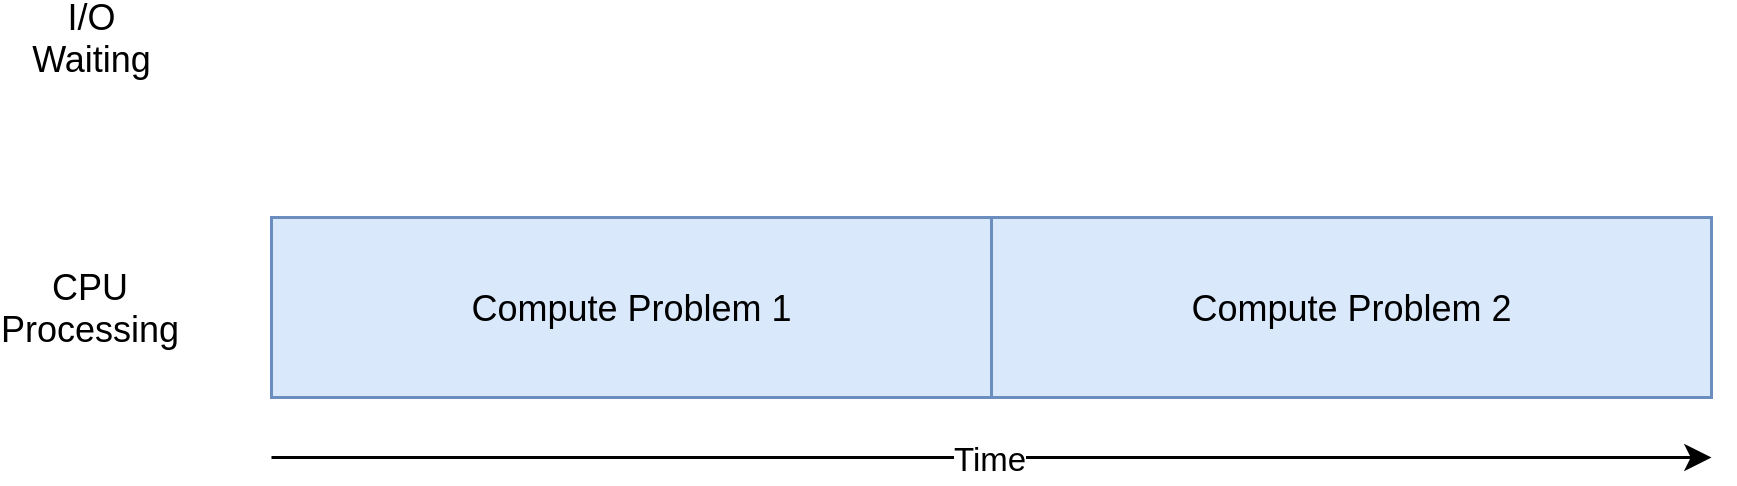
\includegraphics{../figures/CPUBound.png}
            \caption{A diagram for a CPU-intensive program. Blue boxes show time when the program is doing work.}
        \end{figure}

    \end{frame}


    \begin{frame}
        \frametitle{I/O-bound tasks: threading, asynchronicity}

        \begin{itemize}
            \item Only one process (in Python)
            \item Not \emph{really} simultaneous: but can sometimes fake it quite well
            \item Good for: sending requests (to DB, to APIs), waiting for user input, etc.
        \end{itemize}

    \end{frame}


    \begin{frame}
        \frametitle{Threading}

        \begin{itemize}
            \item A \textbf{thread} of execution is the smallest sequence of programmed
            instructions that can be managed independently by a scheduler, which is typically a part of the operating system.
            \item Pre-emptive multitasking: the system (scheduler) interrupts threads at arbitrary moments,
            switches to another thread, and later resumes the stopped tasks
            \item No task cooperation is necessary
            \item Caveats: Race conditions! $\Rightarrow random bugs. Thread-safety is important!
        \end{itemize}

    \end{frame}


    \begin{frame}
        \frametitle{Asynchronicity}

        \begin{itemize}
            \item Event loop -- definition
            \item Cooperative multitasking: tasks have to be programmed to yield control when
            they don't need system resources $\Rightarrow$ easier resources sharing
            \item What if a task does not cooperate? -- blocking operations
        \end{itemize}

    \end{frame}



    %%%%%%%%%%%%%%%%%%%%%%%%%%%%%%%%%%%%%%%%%%%%%%%%
    \section{Concurrency in Python}

    \begin{frame}
        \frametitle{Built-ins}

        \begin{itemize}
            \item \texttt{multiprocessing} -- for CPU-bound tasks
            \item \texttt{threading}  -- \dots?
            \item \texttt{asyncio} -- from Python 3.4 on
        \end{itemize}

    \end{frame}

    \begin{frame}
        \frametitle{Examples!}


    \end{frame}


    \section{GIL}

    \begin{frame}
        \frametitle{Global Interpreter Lock}

        \begin{itemize}
            \item The mechanism used by the CPython interpreter to assure that only one thread executes Python bytecode at a time
            \item But why?!
            \item Makes the object model implicitly safe against concurrent access
            \item Reference counting -- instead of garbage collection; (more about it in the next slide)
        \end{itemize}

    \end{frame}

    \begin{frame}[fragile]
        \frametitle{Global Interpreter Lock -- continued}

        Reference counting:
        any reference to an object modifies it (or at least its refcount)
        \begin{verbatim}
            > import sys
            > a = []
            > sys.getrefcount(a)
            2
            > b = a
            > sys.getrefcount(a)
            3
        \end{verbatim}
    \end{frame}

    \begin{frame}
        \frametitle{Global Interpreter Lock -- continued}
        \begin{itemize}
            \item The reference count needs protection against race conditions!
            \item Otherwise: memory leaks (never released) or incorrectly released memory,
            while a reference to the object still exist
            \item \textbf{A solution?} Add locks to all the objects that are shared between threads
            \item \emph{Consequences:} decreased performance, and deadlocks!
            \item \textbf{A better solution?} A single lock: execution of any Python code
            requires acquiring the lock on the interpreter
            \item \emph{Consequences:} easier, thread-safe, but any CPU-bound program becomes, effectively, single-threaded.
            \item Back then, when Python was a young language, it made it easy to add C extensions
            (didn't have to be thread-safe) -- this helped make Python more popular
        \end{itemize}

    \end{frame}

    \begin{frame}
        \frametitle{Global Interpreter Lock -- continued}


        The GIL is always released when doing I/O.

        \begin{quotation}
            [O]nly the thread that has acquired the GIL may operate on Python objects or
            call Python/C API functions. In order to emulate concurrency of execution,
            the interpreter regularly tries to switch threads (\dots).
            The lock is also released around potentially blocking I/O operations like
            reading or writing a file, so that other Python threads can run in the meantime.
        \end{quotation}

    \end{frame}

    \begin{frame}
        \frametitle{Global Interpreter Lock -- continued}

        How to deal with GIL?
        \begin{itemize}
            \item multithreading $\rightarrow$ asyncio
            \item multithreading $\rightarrow$ multiprocessing (+ asyncio)
            \item CPU-intensive functions $\rightarrow$ Cython (no GIL!)
            \item Python $\rightarrow$ a faster language\dots?
        \end{itemize}

        Pycharm: concurrency diagrams (reveals locking issues, but omits GIL)

    \end{frame}

    %\begin{frame}
    %    \frametitle{}
    %
    %\end{frame}
    %
    %\begin{frame}
    %    \frametitle{}
    %
    %\end{frame}
    %
    %\begin{frame}
    %    \frametitle{}
    %
    %\end{frame}
    %
    %\begin{frame}
    %    \frametitle{}
    %
    %\end{frame}

    \begin{frame}
        \frametitle{Concurrency in Python -- bibliography \& further reading}

        \begin{itemize}
            \item<1-> Jim Anderson, \emph{"Speed Up Your Python Program With Concurrency"},
            \texttt{https://realpython.com/python-concurrency/}
            \item<1-> David Beazley, \emph{"An Introduction to Python Concurrency"},
                presented at USENIX Technical ConferenceSan Diego, June, 2009.
                Slides available at \texttt{https://speakerd.s3.amazonaws.com/presentations/
            3770713233254908b259542c4361e976/Concurrent.pdf}
        \end{itemize}
    \end{frame}

    \begin{frame}
        \frametitle{GIL -- bibliography \& further reading}
        \begin{itemize}
            \item<1-> Abhinav Ajitsaria, \emph{"What is the Python Global Interpreter Lock (GIL)?"}
            \texttt{https://realpython.com/python-gil/}
            \item<1-> Python Wiki, \emph{"Global Interpreter Lock"},
            \texttt{https://wiki.python.org/moin/GlobalInterpreterLock}
%            \footnotesize Discussion of problems with GIL and why it has not been eliminated
            \item<1-> \emph{"Thread State and the Global Interpreter Lock"},
            \texttt{https://docs.python.org/3/c-api/init.html
            \#thread-state-and-the-global-interpreter-lock}
            \item<1-> Christoph Heer, \emph{"Is it me, or the GIL?"}, presented at
            EuroPython 2019 in Basel, Switzerland, July, 2019.
            Slides available at \texttt{https://ep2019.europython.eu/media/conference/
            slides/Lj9n5pc-is-it-me-or-the-gil.pdf}
        \end{itemize}

    \end{frame}

%    \bibliography{main}
%    \bibliographystyle{plain}
%    \begin{thebibliography}
%
%    \bibitem{RealPython}
%    \bibitem{DaBeaz} David Beazley, "An Introduction to Python Concurrency",
%    presented at USENIX Technical ConferenceSan Diego, June, 2009.
%    Slides available at https://speakerd.s3.amazonaws.com/presentations/3770713233254908b259542c4361e976/Concurrent.pdf
%    \end{thebibliography}


\end{document}
